{\em Auteur: Laura Vranken}\\

\noindent
De Drone Autopilot bepaalt de positie van de drone relatief ten opzichte van zijn doel a.d.h.v. twee beelden gegeneerd door de dronecamera's. Bovendien zorgt de Autopilot ervoor dat de drone juist naar zijn doel toe vliegt. De drone bereikt zijn doel wanneer hij door een gekleurde bol gevlogen is of door ze allemaal in geval van meerdere bollen.  Daarnaast moet de Autopilot ook rekening houden met een mogelijke invloed van wind die de drone van zijn koers doet afwijken en ook met obstakels waarrond hij moet vliegen.
\\
\\
Ten eerste moeten de beelden die de Autopilot van de Virtual Testbed binnenkrijgt, geanalyseerd worden. Dit gebeurt door iteratief de kleurwaarden van elke pixel te vergelijken met de waarde van de opgegeven kleur indien er al een doel beslist is. Anders zullen de pixels gegroepeerd worden per kleur dat voorkomt in een HashMap. De gekleurde pixels worden bijgehouden door hun positie ten opzichte van het beeld, uitgedrukt in rij en kolom, op te slaan. We baseren onze berekeningen op het midden van de bol. Dit kan benaderd worden op twee manieren: via het zwaartepunt of de kleinste-kwadratenmethode op de randpunten van de cirkel. Het zwaartepunt van een bepaalde kleur pixels is te berekenen via het gemiddelde van de opgeslagen co\"ordinaten. De kleinste-kwadratenmethode zoekt daarentegen eerst de randpunten uit van de cirkel. Deze worden vervolgens gebruikt in een algoritme, dat de cirkel bepaalt die het beste past in de gegeven randpunten. Hieruit kan dan de positie van het centrum van de bol bepaald worden. \cite{website:kleinsteKwadraten} De Autopilot zal eerst gebruik maken van de kleinste-kwadratenmethode en overschakelen op de zwaartepuntberekening wanneer er onvoldoende randpunten zijn, aangezien deze minder nauwkeurig is wanneer het middelpunt buiten beeld ligt.
TODO: Vincent moet bij algoritmen zijn kleinste kwadraten meer uitleggen!
\\
Indien de Autopilot geen gekleurde pixels detecteert, zal de drone geleidelijkaan de wereld afscannen. Hierover meer info in subsectie \ref{subsec: PI Controllers}.
\\
\\
Wanneer de Autopilot iets in beeld gekregen heeft, zal hij starten met zijn positie relatief tegenover zijn doel te bepalen. Dit gebeurt in volgende stappen.
\\
Ten eerst wordt de diepte bepaald. Dit kan met behulp van de formule van stereo vision \cite{website:techbriefs} uitgewerkt worden.
Zie Figuur \ref{fig:DiepteberekeningDroneEnDoel} voor een grafische weergave van de berekening. Z stelt de diepte [m] voor, c de afstand [m] tussen de camera's, f de focale afstand [pixel] en $x_1$ en $x_2$ stellen de afstand [pixel] voor tussen het middelpunt van het beeld en het middelpunt van de bol op het beeld voor.
\begin{figure}[h]
	\centering
	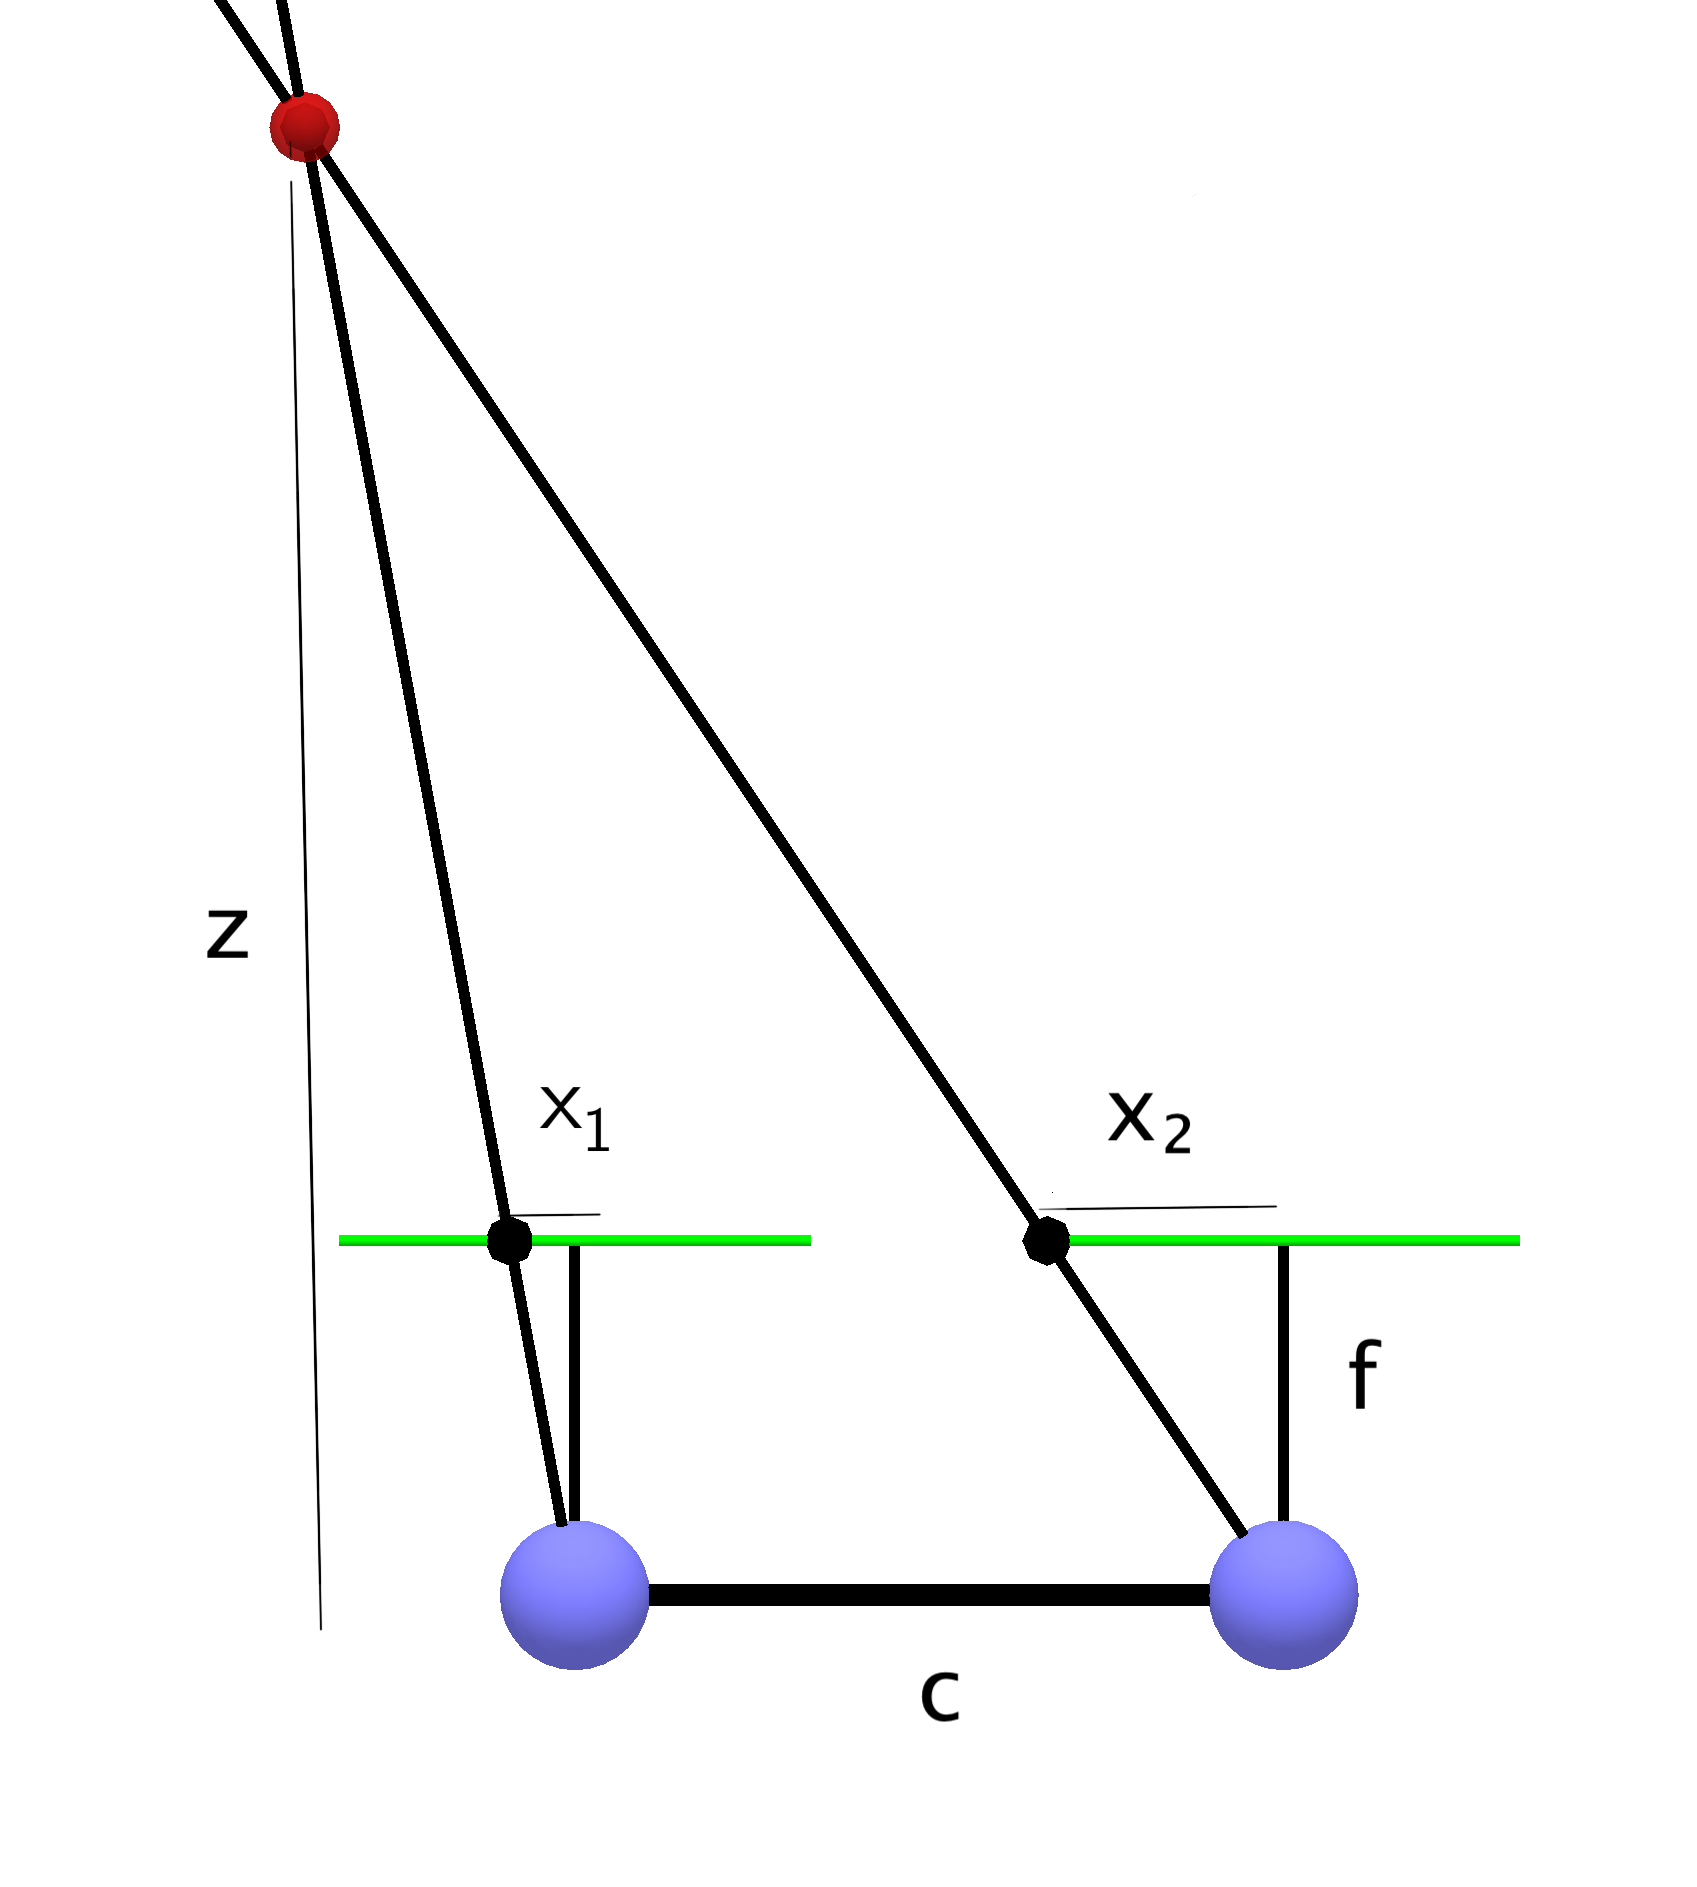
\includegraphics[width=0.3\textwidth]{DiepteberekeningDroneEnDoel.png}
	\caption{Diepteberekening tussen drone en doel. In formulevorm: \(Z = \frac{c * f}{x_1 - x_2}\).}
	\label{fig:DiepteberekeningDroneEnDoel}
\end{figure}
\\
Vervolgens bepalen we de fout op de horizontale hoek, $\alpha$. Hiermee wordt de afwijking tussen de horizontale positie van de bol en het midden van de drone bedoeld. Deze formule wordt afgeleid via de goniometrische regels. Zie Figuur \ref{fig:RelatieveHorizontaleHoek} voor grafische ondersteuning. De hoek $\delta$ stelt hier de helft van de horizontale hoek die het beeld overspant, voor en b stelt de helft van de breedte van het beeld voor. Onder de figuur, kan eveneens ook de uitwerking van de formule gevonden worden.
\\
Tenslotte bepalen we ook de fout op de verticale hoek, $\beta$. Dit is de afwijking van de hoogte van de bol ten opzichte van de hoogte van de drone. Wederom afgeleid via de goniometrie en weergegeven in Figuur \ref{fig:RelatieveVerticaleHoek}, met $y_2$ de verticale afstand [pixel] tussen de het middelpunt van het beeld en het middelpunt van de bol.
\begin{figure}[h]
	\centering
	\begin{minipage}{.45\textwidth}
		\centering
		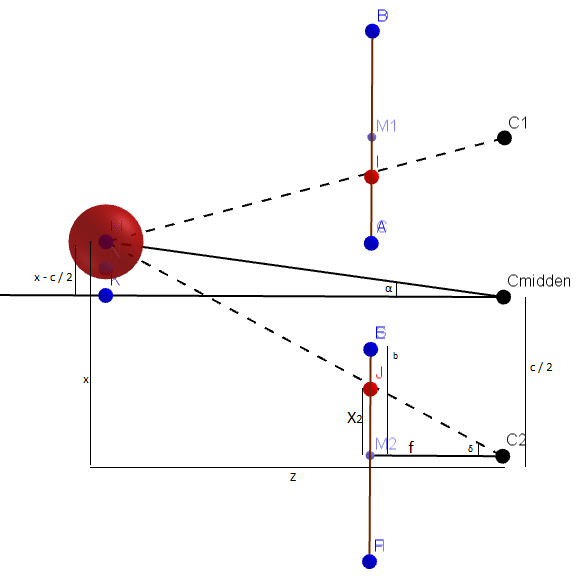
\includegraphics[width=0.8\textwidth]{RelatieveHorizontaleHoek.png}
		\caption{Relatieve horizontale hoek.}
		\label{fig:RelatieveHorizontaleHoek}
	\end{minipage}
	\begin{minipage}{.45\textwidth}
		\centering
		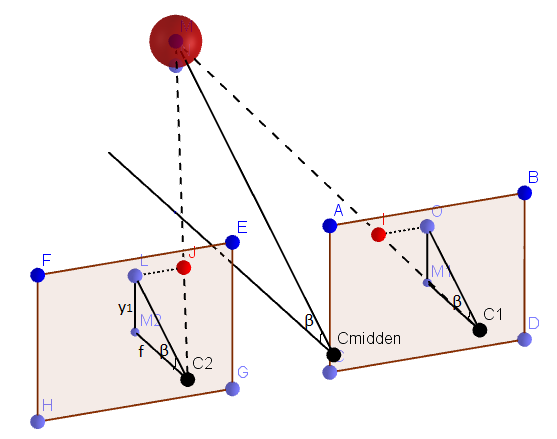
\includegraphics[width=0.96\textwidth]{RelatieveVerticaleHoek.png}
		\caption{Relatieve verticale hoek.}
		\label{fig:RelatieveVerticaleHoek}
	\end{minipage}%
	\caption*{In Figuur \ref{fig:RelatieveHorizontaleHoek} wordt de relatieve horizontale hoek tussen drone en doel weergegeven door \(\tan(\alpha) = \frac{x-\frac{c}{2}}{Z}\), voor de volledige uitwerking zie formule \ref{eq:RelatieveVerticaleHoekBegin} tot \ref{eq:RelatieveVerticaleHoekEind}.\\
		In Figuur \ref{fig:RelatieveVerticaleHoek} wordt de relatieve verticale hoek weergegeven tussen drone en doel. De relatie wordt gegeven door volgende formule: \(\tan(\beta) = \frac{y_1}{f}\).}
\end{figure}
\begin{figure}[h]
	\centering
	\begin{minipage}{.5\textwidth}
		Berekening brandpuntsafstand f:
		\begin{equation} \label{eq:RelatieveVerticaleHoekBegin}
		\tan(\delta) = \frac{b}{f}
		\end{equation}
		\begin{equation} 
		f = \frac{b}{\tan(\delta)}
		\end{equation}
	\end{minipage}
	\begin{minipage}{.45\textwidth}
		Berekening afstand x:
		\begin{equation} 
		\frac{x_2}{f} = \frac{x}{z}
		\end{equation}
		\begin{equation} \label{eq:RelatieveVerticaleHoekEind}
		x = z * \frac{x_2}{f}	
		\end{equation}
	\end{minipage}%
\end{figure}
\\
Nadat de drone zijn positie bepaald heeft, kan hij zijn fouten (horizontale en verticale hoek en eventuele roll) bijsturen a.d.h.v. PI controllers die beslissen over respectievelijk yaw, thrust en roll bewegingen. Meer info over de werking van de controllers wordt gegeven in subsectie \ref{subsec: Scannen wereld}.
\\
\\
Nu rest er ons enkel nog de pitch te bepalen zodat we onder een ingestelde thrust voorwaarts richting de bol kunnen bewegen. Het eerste idee was om dit op basis van een soort van snelheidscontroller te doen, aangezien de snelheid afhankelijk is van de pitch en dat we hierdoor ook de snelheid konden controlleren en laag houden. De snelheid is echter niet te bepalen door de onbekende windkrachten of door de numeriek wiskundige beperkingen op afgeleiden berekenen. Bijgevolg zijn we overgegaan op het tweede plan. Dit plan houdt in dat de drone pitcht met een rate op basis van een afstandscontroller, zodat hij een kleine afstand overbrugt, terug recht komt wat de snelheid een klein beetje afbouwt en dan weer opnieuw pitcht om verder te gaan. Wanneer er tegenwind is, zal de afstandscontroller de drone toelaten om verder te pitchen om toch op zijn doel te raken.
\\
\\
Tenslotte moet dit proces herhaaldelijk worden uitgevoerd ten gevolge van de invloed van wind. De wind kan de drone namelijk uit koers brengen. Hierdoor zal de drone telkens zijn positie moeten herberekenen en zich opnieuw ori\"enteren en de controllers laten bijsturen.
\\
De bijkomstige moeilijkheid van obstakels zal verder worden uitgewerkt in subsectie \ref{subsec: Obstakels}.

\subsubsection{Scannen wereld}
\label{subsec: Scannen wereld}
\input{scannenWereld.tex}

\subsubsection{PI Controllers}
\label{subsec: PI Controllers}
\noindent
Om een PI-controller te kunnen gebruiken, is het belangrijk om te weten wat het is en wat het doet. Zoals in \cite{website:PIDController} wordt aangegeven, fungeert de controller als een controlelus-feedback mechanisme. Dit systeem gaat proberen de afwijking op de meetwaarde te corrigeren. Het berekent namelijk continu de foutwaarde \(e(t)\) als het verschil tussen de correcte waarde en de gemeten waarde. Op basis van deze gegevens berekent de controller de nodige correctie.
\\
\\
Er is gekozen voor een PI-controller i.p.v. een PID-controller, aangezien die ook in de meeste re\"ele systemen gebruikt wordt. Bovendien is de term D (Derivative) heel gevoelig aan ruis en zou die een bijkomende moeilijkheid vormen om af te stellen.
\\
PI staat voor Proportional-Integral. Het P-deel zorgt ervoor dat het verschil in gewenste waarde en de gemeten waarde met een factor $K_p$ wordt versterkt. 
I zorgt voor een constante sommatie van de afwijking en vergroot de correctiewaarde afhankelijk van hoelang er een afwijking bestaat tussen gemeten en gewenste waarde. Dit wordt met een factor $K_i$ versterkt. Deze constanten worden manueel bepaald door de reactie van de controller uit te plotten in grafieken en hun gedrag te optimaliseren door deze co\"effici\"enten aan te passen.
\\
\\
De correctie kan berekend worden op basis van formule \ref{eq: PI}.
\begin{equation} \label{eq: PI}
	u(t) = K_p * e(t) + K_i * \int e(t) dt
\end{equation}
Hier is \(u(t)\) de correctie, $K_p$ de proportional constante, $K_i$ de integral constante en \(e(t)\) de foutwaarde op tijdstip \(t\).
\\
\\
Voorgaande theorie wordt toegepast op dit project.
\\
Ten eerste wordt de roll-controller bekeken. Hij heeft als doel de roll gelijk aan nul te houden. Dit is dan ook ineens de gewenste waarde. De controller begint slechts bij te sturen wanneer de gemeten roll waarde groter is dan \(0.2\degree\) in positieve of negatieve zin. Bijsturen gebeurt door de correctiewaarde als input te nemen voor de rollrate.
\\
Vervolgens is er een yaw-controller. Deze werkt enkel wanneer het doel in beeld is, aangezien de drone een ori\"entatiepunt nodig heeft om de yaw te kunnen bepalen. De gewenste waarde is gelijk aan een horizontale afwijking $\alpha$ van nul graden. De controller gaat dit bijsturen op dezelfde manier als bij de roll-controller.
\\
De height-controller stelt de thrustwaarde in en verschilt licht van de anderen doordat hij de correctiewaarde optelt bij de standaard waarde om de zwaartekracht tegen te gaan. Verder probeert hij de verticale afwijking naar nul te herleiden.
\\
De pitch-controller wordt gebruikt om zo snel mogelijk te kunnen hoveren en dus een pitch van nul te krijgen. Dit gebeurt op dezelfde manier als voorgaande controllers.
\\
Ten slotte is er ook nog een distance-controller. Deze gaat proberen de afstand naar nul te reduceren met stappen van \(0.1\)m en helpt bij het voorwaarts vliegen om de pitchrate in te stellen, zoals uitgelegd in sectie \ref{subsec: Vliegstrategie}.

\subsubsection{Obstakels}
\label{subsec: Obstakels}
\noindent
De laatste hindernis is het ontwijken van obstakels. De eerste taak is het bepalen van de positie van de obstakels. Dit gebeurt door eerst de verschillende tinten grijs uit het beeld te filteren en vervolgens de obstakels te verwijderen die niet in de buurt van onze vliegrichting liggen. Tenslotte wordt de dichtste eruit gekozen, aangeziene die als eerste moet worden ontweken.
\\
\\
Het ontwijken zelf gebeurt a.d.h.v. de hoogte controller. Indien de bol in de bovenste helft van het beeld staat, zal de drone onder de bol doorvliegen. Indien de bol in de onderste helft van het beeld staat, zal hij erover vliegen. Er wordt geopteerd voor deze strategie aangezien de reactie op de thrust vrij snel en accuraat is. De andere optie is er naast vliegen. Dit zou veel moeilijker en onvoorspelbaarder zijn daar de drone nog voorwaarts zou verder drijven, ook al is de yaw reeds aangepast. De roll aanpassen, biedt een oplossing, maar is een moeilijke opdracht. Dit verantwoordt de keuze om de hoogte aan te passen.


















